% =====================================================================
% Clase -- Geometría 10° -- Trimestre I -- Semana 04
% Sesión 003 (lun 21 sep., 13:00, 40 min)
% Tema: Distancia entre dos puntos
% Subtema: La fórmula de la distancia a partir del teorema de Pitágoras
% Hilo conductor del trimestre I: «Ubicarse en la Tierra: de las coordenadas geográficas al
% plano cartesiano»
% Tema 2 de la guía: Distancia entre dos puntos (tema:distancia)
% Material del docente (no se entrega a los estudiantes).
% =====================================================================
\documentclass[11pt]{article}
\makeatletter\def\input@path{{../../../../../plantillas/estilo/}}\makeatother
\usepackage{mmcantillo}
\guiadelestudiante{../../guia-didactica/guia-periodo-I-geometria-analitica}

\tipodocumento{Clase}
\asignatura{Geometría}
\titulo{Semana 4: medir sin regla}
\grado{10°}
\periodo{I}

% DBA: matematicas grado 10 · DBA 5 — Explora y describe las propiedades de los lugares
% geométricos y de sus transformaciones a partir de diferentes representaciones. Evidencia de
% esta sesión: deducir y usar la expresión de la distancia entre dos puntos como herramienta
% para describir lugares geométricos (la circunferencia y la mediatriz de las sesiones 005-006
% se definen con ella).

\begin{document}

\encabezado*

\begin{center}
{\renewcommand{\arraystretch}{1.3}
\begin{tabularx}{\linewidth}{@{}l l l X l@{}}
  \toprule
  \textbf{Sesión} & \textbf{Fecha} & \textbf{Min} & \textbf{Subtema} & \textbf{Entregables}\\
  \midrule
  003 & lun 21 sep., 13:00 & 40 & La fórmula de la distancia desde Pitágoras
      & Se deja tarea (5 puntos)\\
  \bottomrule
\end{tabularx}}
\end{center}

Segundo paso del hilo: en la sesión anterior ubicamos puntos con coordenadas, como en un mapa.
Hoy respondemos la pregunta que hace útil ese mapa —\emph{¿qué tan lejos están dos puntos?}—
y resulta que la respuesta es el teorema de Pitágoras de siempre, escrito con coordenadas.
Referencia: \refguia{tema:distancia}.

% ---------------------------------------------------------------------
\seccion{Sesión 003 — lunes 21 de septiembre · 13:00 · 40 min}

\textbf{Objetivo.} Deducir la fórmula de la distancia entre dos puntos como un caso del
teorema de Pitágoras y aplicarla para decidir propiedades de una figura (lados iguales,
tipo de triángulo) con números en vez de con la regla.

\textbf{Materiales.} Tablero cuadriculado o cuadrícula dibujada; regla; la guía.

\begin{center}
{\renewcommand{\arraystretch}{1.3}
\begin{tabularx}{\linewidth}{@{}l l X@{}}
  \toprule
  \textbf{Momento} & \textbf{Min} & \textbf{Actividad}\\
  \midrule
  Enganche & 0--5 & Dos puntos en la cuadrícula, $A(2,3)$ y $B(6,6)$. «Mídanlo con la
    regla.» Salen respuestas distintas. «¿Y si el plano fuera un mapa de Colombia y no
    tuviéramos regla?»\\
  Deducción & 5--18 & Trazar el triángulo rectángulo con catetos horizontal y vertical:
    los catetos miden $|x_2 - x_1|$ y $|y_2 - y_1|$, y la distancia es la hipotenusa.
    Escribir $d = \sqrt{(x_2-x_1)^2 + (y_2-y_1)^2}$ y comprobar con $A$ y $B$: $\sqrt{16+9}
    = 5$. Insistir: \textbf{no es una fórmula nueva}, es Pitágoras con coordenadas.\\
  Dos cuidados & 18--26 & (1) El valor absoluto sobra porque va al cuadrado: por eso da lo
    mismo restar en un orden o en el otro. (2) El error de siempre: restar mal cuando hay
    negativos, $4 - (-2) = 6$ y no $2$. Hacer un ejemplo con negativos en el tablero.\\
  Aplicación & 26--36 & El triángulo $P(1,1)$, $Q(5,1)$, $R(3,5)$: a ojo parece
    equilátero. Calcular: $PQ = 4$, $QR = PR = 2\sqrt{5} \approx \num{4,47}$. Es isósceles.
    Moraleja del día: la fórmula decide lo que el ojo no distingue.\\
  Cierre & 36--40 & Dejar la tarea. Anuncio: con esta fórmula, la próxima clase definimos
    la circunferencia sin dibujarla —«todos los puntos a la misma distancia de uno fijo».\\
  \bottomrule
\end{tabularx}}
\end{center}

\textbf{Figura para el tablero: la distancia es una hipotenusa.}

\begin{center}
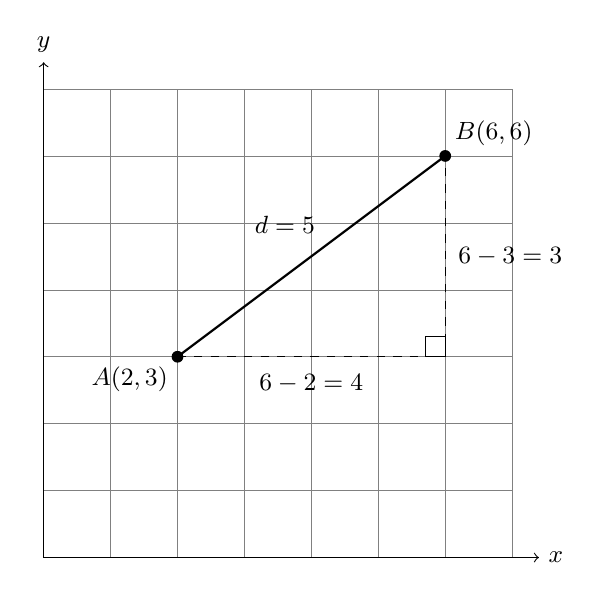
\begin{tikzpicture}[scale=0.85, every node/.style={font=\small}]
  \draw[help lines, step=1] (0,0) grid (7,7);
  \draw[->] (0,0) -- (7.4,0) node[right] {$x$};
  \draw[->] (0,0) -- (0,7.4) node[above] {$y$};
  \coordinate (A) at (2,3); \coordinate (B) at (6,6); \coordinate (C) at (6,3);
  \draw[thick] (A) -- (B);
  \draw[dashed] (A) -- (C) -- (B);
  \draw (5.7,3) rectangle (6,3.3);
  \fill (A) circle (2.5pt) node[below left] {$A(2,3)$};
  \fill (B) circle (2.5pt) node[above right] {$B(6,6)$};
  \node at (4,2.6) {$6-2=4$};
  \node[right] at (6.05,4.5) {$6-3=3$};
  \node[above left] at (4.2,4.7) {$d=5$};
\end{tikzpicture}
\end{center}

\begin{nota}
\textbf{Dónde suele trabarse.} No en la fórmula, sino en la resta con negativos. Si aparece,
vale la pena escribir siempre la resta entre paréntesis —$(x_2 - x_1)$— y leerla en voz alta
antes de operar. La pregunta 4 de la tarea es exactamente ese error, puesto en boca de otra
persona: cuesta menos verlo en el cuaderno ajeno.
\end{nota}

\begin{nota}
\textbf{Si sobra tiempo} (poco probable en 40 min): la aplicación del hilo está en la guía —
un grado de latitud son unos $\qty{111}{km}$, así que con coordenadas geográficas y esta
fórmula se estima la distancia entre dos ciudades. Si no alcanza, queda para el enganche de
la sesión 004.
\end{nota}

\end{document}
